\begin{center}
	\begin{equation} \label{eq:battery_voltage}
		U_\mathrm{B}\left(t\right) =
  		\begin{cases}
   			\left(\dfrac{Q_\mathrm{rem}}{C} + I_\mathrm{C} \, R_2\right) \, \exp \left( -\dfrac{t}{R_2 \, C} \right) + U_0 - I_\mathrm{C} \left( R_1 + R_2 \right) \\ \\
    		\left(\dfrac{Q_\mathrm{rem}}{C} + I_\mathrm{D} \, R_2\right) \, \exp \left( -\dfrac{t}{R_2 \, C} \right) + U_0 - I_\mathrm{D} \left( R_1 + R_2 \right)
  		\end{cases}
	\end{equation} 
\end{center}

\begin{center}
	\begin{equation} \label{eq:parameters_r_1}
		R_1 = \left( a_1 + a_2 \, x + a_3 \, x^2 \right) \, \exp\left( - a_4 \, y \right) + a_5 + a_6 \, x + a_7 \, x^2
	\end{equation} 
\end{center}

\begin{center}
	\begin{equation} \label{eq:parameters_r_2}
		R_2 = \left( a_8 + a_9 \, x + a_{10} \, x^2 \right) \, \exp\left( - a_{11} \, y \right) + a_{12} + a_{13} \, x + a_{14} \, x^2
	\end{equation} 
\end{center}

\begin{center}
	\begin{equation} \label{eq:parameters_c}
		C = - \left( a_{15} + a_{16} \, x + a_{17} \, x^2 \right) \, \exp\left( - a_{18} \, y \right) + a_{19} + a_{20} \, x + a_{21} \, x^2
	\end{equation} 
\end{center}

\begin{center}
	\begin{equation} \label{eq:parameters_u_0}
		\begin{aligned} 
		U_0 = \left( a_{22} + a_{23} \, x + a_{24} \, x^2 \right) \, \exp\left( - a_{25} \, y \right) + a_{26} + a_{27} \, y + &a_{28} \, y^2 + a_{29} \, y^3 \\ &- a_{30} \, x + a_{31} \, x^2
		\end{aligned}
	\end{equation} 
\end{center}

\begin{center}
	\begin{equation} \label{eq:battery_x}
		x =
  		\begin{cases}
   			\dfrac{I_\mathrm{C}}{Q_\mathrm{rem}} \\ \\
			\dfrac{I_\mathrm{D}}{Q_\mathrm{rem}}
  		\end{cases}
	\end{equation} 
\end{center}

\begin{center}
	\begin{equation} \label{eq:battery_y}
		y =
  		\begin{cases}
   			\mathrm{SOC_{cr}} \\
			\mathrm{1 - DOD_{cr}}
  		\end{cases}
	\end{equation} 
\end{center}

\begin{figure}[h!]
	\centering
	

\tikzset{every picture/.style={line width=0.75pt}} %set default line width to 0.75pt        

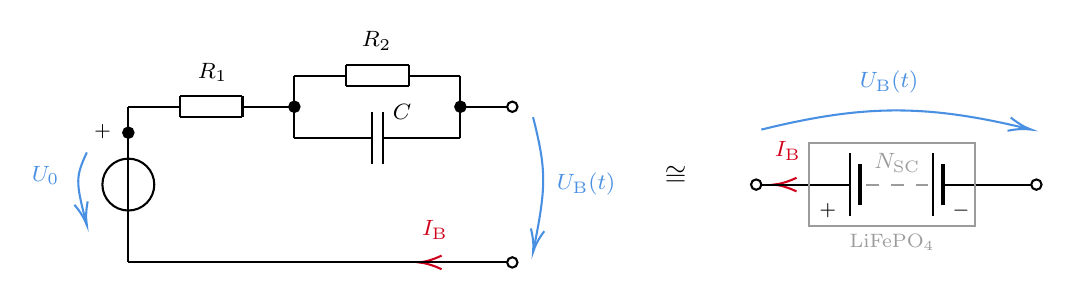
\begin{tikzpicture}[x=0.75pt,y=0.75pt,yscale=-1,xscale=1]
%uncomment if require: \path (0,440); %set diagram left start at 0, and has height of 440

%Straight Lines [id:da5486306098865306] 
\draw [color={rgb, 255:red, 208; green, 2; blue, 27 }  ,draw opacity=1 ]   (406,107.5) -- (393,107.5) ;
\draw [shift={(391,107.5)}, rotate = 360] [color={rgb, 255:red, 208; green, 2; blue, 27 }  ,draw opacity=1 ][line width=0.75]    (10.93,-3.29) .. controls (6.95,-1.4) and (3.31,-0.3) .. (0,0) .. controls (3.31,0.3) and (6.95,1.4) .. (10.93,3.29)   ;
%Straight Lines [id:da03626976474172294] 
\draw    (489.5,107.5) -- (515,107.5) ;
%Straight Lines [id:da4469958263298277] 
\draw    (385,107.5) -- (410.5,107.5) ;
%Straight Lines [id:da40108610575226744] 
\draw [line width=0.75]    (427.5,92.5) -- (427.5,122.5) ;
%Straight Lines [id:da8088791201907699] 
\draw [color={rgb, 255:red, 155; green, 155; blue, 155 }  ,draw opacity=1 ] [dash pattern={on 4.5pt off 4.5pt}]  (465.5,107.5) -- (430.5,107.5) ;
%Straight Lines [id:da8015404215815611] 
\draw [line width=1.5]    (432.5,97.5) -- (432.5,117.5) ;
%Straight Lines [id:da26803317980125607] 
\draw [line width=0.75]    (467.5,92.5) -- (467.5,122.5) ;
%Straight Lines [id:da19235798370580381] 
\draw [line width=1.5]    (472.5,97.5) -- (472.5,117.5) ;
%Straight Lines [id:da7275713458105508] 
\draw    (427.5,107.5) -- (410.5,107.5) ;
%Straight Lines [id:da5198817320251647] 
\draw    (489.5,107.5) -- (472.5,107.5) ;
%Shape: Rectangle [id:dp3168250836016058] 
\draw  [color={rgb, 255:red, 155; green, 155; blue, 155 }  ,draw opacity=1 ] (488,87.5) -- (488,127.5) -- (408,127.5) -- (408,87.5) -- cycle ;
%Shape: Circle [id:dp7331821401896568] 
\draw   (515,107.5) .. controls (515,106.12) and (516.12,105) .. (517.5,105) .. controls (518.88,105) and (520,106.12) .. (520,107.5) .. controls (520,108.88) and (518.88,110) .. (517.5,110) .. controls (516.12,110) and (515,108.88) .. (515,107.5) -- cycle ;
%Shape: Circle [id:dp6031096460656484] 
\draw   (380,107.5) .. controls (380,106.12) and (381.12,105) .. (382.5,105) .. controls (383.88,105) and (385,106.12) .. (385,107.5) .. controls (385,108.88) and (383.88,110) .. (382.5,110) .. controls (381.12,110) and (380,108.88) .. (380,107.5) -- cycle ;
%Straight Lines [id:da10162123830846292] 
\draw    (135,75) -- (135,65) ;
%Straight Lines [id:da09071387753404836] 
\draw    (105,75) -- (105,65) ;
%Straight Lines [id:da6551313002354882] 
\draw    (105,65) -- (135,65) ;
%Straight Lines [id:da6708661444464734] 
\draw    (105,75) -- (135,75) ;
%Curve Lines [id:da4412878233471469] 
\draw [color={rgb, 255:red, 74; green, 144; blue, 226 }  ,draw opacity=1 ]   (60,92) .. controls (54.66,103.64) and (54.5,105.87) .. (59.52,125.16) ;
\draw [shift={(60,127)}, rotate = 255.32] [color={rgb, 255:red, 74; green, 144; blue, 226 }  ,draw opacity=1 ][line width=0.75]    (10.93,-3.29) .. controls (6.95,-1.4) and (3.31,-0.3) .. (0,0) .. controls (3.31,0.3) and (6.95,1.4) .. (10.93,3.29)   ;
%Straight Lines [id:da9000234956108482] 
\draw [color={rgb, 255:red, 208; green, 2; blue, 27 }  ,draw opacity=1 ]   (235,145) -- (222,145) ;
\draw [shift={(220,145)}, rotate = 360] [color={rgb, 255:red, 208; green, 2; blue, 27 }  ,draw opacity=1 ][line width=0.75]    (10.93,-3.29) .. controls (6.95,-1.4) and (3.31,-0.3) .. (0,0) .. controls (3.31,0.3) and (6.95,1.4) .. (10.93,3.29)   ;
%Straight Lines [id:da3416487864826865] 
\draw    (80,120) -- (80,145) ;
%Shape: Circle [id:dp5241884850752403] 
\draw   (67.5,107.5) .. controls (67.5,100.6) and (73.1,95) .. (80,95) .. controls (86.9,95) and (92.5,100.6) .. (92.5,107.5) .. controls (92.5,114.4) and (86.9,120) .. (80,120) .. controls (73.1,120) and (67.5,114.4) .. (67.5,107.5) -- cycle ;
%Straight Lines [id:da04046304764089448] 
\draw    (80,95) -- (80,120) ;
%Shape: Circle [id:dp07300379742123142] 
\draw  [fill={rgb, 255:red, 0; green, 0; blue, 0 }  ,fill opacity=1 ] (157.5,70) .. controls (157.5,68.62) and (158.62,67.5) .. (160,67.5) .. controls (161.38,67.5) and (162.5,68.62) .. (162.5,70) .. controls (162.5,71.38) and (161.38,72.5) .. (160,72.5) .. controls (158.62,72.5) and (157.5,71.38) .. (157.5,70) -- cycle ;
%Shape: Circle [id:dp3711379210458987] 
\draw   (262.5,145) .. controls (262.5,143.62) and (263.62,142.5) .. (265,142.5) .. controls (266.38,142.5) and (267.5,143.62) .. (267.5,145) .. controls (267.5,146.38) and (266.38,147.5) .. (265,147.5) .. controls (263.62,147.5) and (262.5,146.38) .. (262.5,145) -- cycle ;
%Shape: Circle [id:dp3878328782765075] 
\draw   (262.5,70) .. controls (262.5,68.62) and (263.62,67.5) .. (265,67.5) .. controls (266.38,67.5) and (267.5,68.62) .. (267.5,70) .. controls (267.5,71.38) and (266.38,72.5) .. (265,72.5) .. controls (263.62,72.5) and (262.5,71.38) .. (262.5,70) -- cycle ;
%Curve Lines [id:da09021451478739229] 
\draw [color={rgb, 255:red, 74; green, 144; blue, 226 }  ,draw opacity=1 ]   (275,75) .. controls (281.37,100.48) and (281.5,107.71) .. (275.38,138.11) ;
\draw [shift={(275,140)}, rotate = 281.48] [color={rgb, 255:red, 74; green, 144; blue, 226 }  ,draw opacity=1 ][line width=0.75]    (10.93,-3.29) .. controls (6.95,-1.4) and (3.31,-0.3) .. (0,0) .. controls (3.31,0.3) and (6.95,1.4) .. (10.93,3.29)   ;
%Straight Lines [id:da69845637987507] 
\draw    (80,145) -- (262.5,145) ;
%Straight Lines [id:da9530219860330629] 
\draw    (105,70) -- (80,70) ;
%Straight Lines [id:da13641497247136147] 
\draw    (160,70) -- (135,70) ;
%Straight Lines [id:da3222344945770197] 
\draw    (160,55) -- (160,85) ;
%Straight Lines [id:da03154461116871499] 
\draw    (215,60) -- (215,50) ;
%Straight Lines [id:da9178214100407323] 
\draw    (185,60) -- (185,50) ;
%Straight Lines [id:da9202821298731263] 
\draw    (185,50) -- (215,50) ;
%Straight Lines [id:da6804485009486552] 
\draw    (185,60) -- (215,60) ;
%Straight Lines [id:da44637908280074057] 
\draw    (240,55) -- (215,55) ;
%Shape: Circle [id:dp2998085410898652] 
\draw  [fill={rgb, 255:red, 0; green, 0; blue, 0 }  ,fill opacity=1 ] (237.5,70) .. controls (237.5,68.62) and (238.62,67.5) .. (240,67.5) .. controls (241.38,67.5) and (242.5,68.62) .. (242.5,70) .. controls (242.5,71.38) and (241.38,72.5) .. (240,72.5) .. controls (238.62,72.5) and (237.5,71.38) .. (237.5,70) -- cycle ;
%Straight Lines [id:da4638066263785239] 
\draw    (240,85) -- (202.5,85) ;
%Straight Lines [id:da6248762173296205] 
\draw    (240,55) -- (240,85) ;
%Straight Lines [id:da7917075398915874] 
\draw    (197.5,72.5) -- (197.5,97.5) ;
%Straight Lines [id:da8107069018392383] 
\draw    (202.5,72.5) -- (202.5,97.5) ;
%Straight Lines [id:da45783914390262104] 
\draw    (197.5,85) -- (160,85) ;
%Straight Lines [id:da5004670157456534] 
\draw    (262.5,70) -- (240,70) ;
%Straight Lines [id:da3627490634310542] 
\draw    (80,70) -- (80,95) ;
%Shape: Circle [id:dp1840781654633079] 
\draw  [fill={rgb, 255:red, 0; green, 0; blue, 0 }  ,fill opacity=1 ] (77.5,82.5) .. controls (77.5,81.12) and (78.62,80) .. (80,80) .. controls (81.38,80) and (82.5,81.12) .. (82.5,82.5) .. controls (82.5,83.88) and (81.38,85) .. (80,85) .. controls (78.62,85) and (77.5,83.88) .. (77.5,82.5) -- cycle ;
%Straight Lines [id:da6101761358252291] 
\draw    (185,55) -- (160,55) ;
%Curve Lines [id:da9577142414197803] 
\draw [color={rgb, 255:red, 74; green, 144; blue, 226 }  ,draw opacity=1 ]   (385,81) .. controls (434.5,68.82) and (464.4,68.7) .. (513.51,80.63) ;
\draw [shift={(515,81)}, rotate = 193.82] [color={rgb, 255:red, 74; green, 144; blue, 226 }  ,draw opacity=1 ][line width=0.75]    (10.93,-3.29) .. controls (6.95,-1.4) and (3.31,-0.3) .. (0,0) .. controls (3.31,0.3) and (6.95,1.4) .. (10.93,3.29)   ;

% Text Node
\draw (426,129.9) node [anchor=north west][inner sep=0.75pt]  [font=\scriptsize,color={rgb, 255:red, 0; green, 0; blue, 0 }  ,opacity=1 ]  {$\mathrm{\textcolor[rgb]{0.61,0.61,0.61}{LiFePO}\textcolor[rgb]{0.61,0.61,0.61}{_{4}}}$};
% Text Node
\draw (475.5,114.9) node [anchor=north west][inner sep=0.75pt]  [font=\scriptsize]  {$-$};
% Text Node
\draw (411.5,114.9) node [anchor=north west][inner sep=0.75pt]  [font=\scriptsize]  {$+$};
% Text Node
\draw (438,90.9) node [anchor=north west][inner sep=0.75pt]  [font=\footnotesize,color={rgb, 255:red, 155; green, 155; blue, 155 }  ,opacity=1 ]  {$N_{\mathrm{SC}}$};
% Text Node
\draw (337,97.4) node [anchor=north west][inner sep=0.75pt]  [font=\normalsize]  {$\cong $};
% Text Node
\draw (32,97.4) node [anchor=north west][inner sep=0.75pt]  [font=\footnotesize,color={rgb, 255:red, 74; green, 144; blue, 226 }  ,opacity=1 ]  {$U_{0}$};
% Text Node
\draw (220,123.4) node [anchor=north west][inner sep=0.75pt]  [font=\footnotesize,color={rgb, 255:red, 208; green, 2; blue, 27 }  ,opacity=1 ]  {$I_{\mathrm{B}}$};
% Text Node
\draw (285,100.4) node [anchor=north west][inner sep=0.75pt]  [font=\footnotesize,color={rgb, 255:red, 74; green, 144; blue, 226 }  ,opacity=1 ]  {$U_{\mathrm{B}}( t)$};
% Text Node
\draw (112,47.4) node [anchor=north west][inner sep=0.75pt]  [font=\footnotesize]  {$R_{1}$};
% Text Node
\draw (191,32.4) node [anchor=north west][inner sep=0.75pt]  [font=\footnotesize]  {$R_{2}$};
% Text Node
\draw (206,67.4) node [anchor=north west][inner sep=0.75pt]  [font=\footnotesize]  {$C$};
% Text Node
\draw (62,76.9) node [anchor=north west][inner sep=0.75pt]  [font=\scriptsize]  {$+$};
% Text Node
\draw (431,51.4) node [anchor=north west][inner sep=0.75pt]  [font=\footnotesize,color={rgb, 255:red, 74; green, 144; blue, 226 }  ,opacity=1 ]  {$U_{\mathrm{B}}( t)$};
% Text Node
\draw (390,85.4) node [anchor=north west][inner sep=0.75pt]  [font=\footnotesize,color={rgb, 255:red, 208; green, 2; blue, 27 }  ,opacity=1 ]  {$I_{\mathrm{B}}$};


\end{tikzpicture}

	\caption{Simple electrical equivalent circuit of a $\mathrm{LiFePO}_4$ electrochemical energy storage device. (Recreated from: \cite{})}
	\label{fig:tikz_battery}
\end{figure}
